\subsection{\label{triang}Laser Triangulation}

Triangulation describes a method of determining the location of a point C by measuring the angles $\alpha$ and $\beta$ from two points A and B as well as their distance L, as can be seen in fig. \ref{fig:triang}. The distance d from the baseline between the points A and B is then given by

\begin{eqnarray}
d = \frac{L sin(\alpha)sin(\beta)}{sin(\alpha + \beta)}.
\end{eqnarray}

\begin{figure}[H]
	\centering
	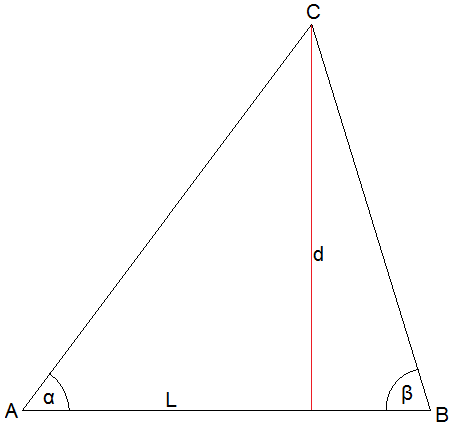
\includegraphics[angle=0,width=0.6\textwidth]{img/triang}
	\caption{Illustration of the basic geometry of determining a distance d by means of triangulation.}
	\label{fig:triang}
\end{figure}

To measure the position of an object by means of laser triangulation, a laser beam is focused on the object. As can be seen in fig. \ref{fig:lasertriang}, the reflected light is collected by a lens and focused onto a position sensitive device (PSD) or a charge-coupled device (CCD). A movement of the object then corresponds to a movement of the laser beam on the detector.\\

The measuring range depends on the size of the PSD as well as on the angle of the beam when being reflected by the object, which is determined by the relative position of PSD and laser. A smaller angle, i.e. a smaller distance between PSD and laser give a larger measuring range, whereas a bigger angle increases the resolution with which the position can be determined.

\begin{figure}[H]
	\centering
	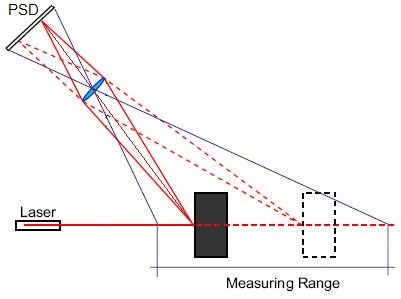
\includegraphics[angle=0,width=0.6\textwidth]{img/lasertriang}
	\caption{Functional principle of laser triangulation.}
	\label{fig:lasertriang}
\end{figure}

\subsection{\label{psd}Position Sensitive Device}

A PSD consists of a photodiode, that releases a current when an incident light beam strikes it. As shown in \ref{fig:psd}, in the case of a one dimensional PSD there are two electrodes attached to each side of the diode. For a two dimensional PSD another two electrodes are attached on the backside of the diode, at 90° angle to the electrode pair on the front.\cite{sitek}\cite{lecturenotes}

%\begin{figure}[H]
%	\centering
%	\includegraphics[angle=0,width=0.6\textwidth]{img/psd}
%	\caption{Scheme of a position sensitive device.}
%	\label{fig:psd}
%\end{figure}

The current caused by the incident photons is divided between the contacts on each side. As the active surface of the photodiode acts as a homogenous resistance, the currents generated depend linearly on the position of the incident light on the PSD. 

\begin{figure}[H]
	\centering
	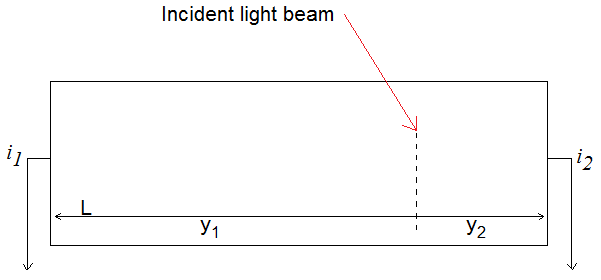
\includegraphics[angle=0,width=0.6\textwidth]{img/psd_calc}
	\caption{.}
	\label{fig:psd2}
\end{figure}

The position $y_2$ as seen in \ref{fig:psd2}can then be obtained by measuring both currents. The sum of the currents $i_1$ and $i_2$ is a constant dependent on the power of the incident light $P_0$ and the sensitivity of the detector $\eta$:

\begin{eqnarray}
i_1 + i_2 = \eta \cdot P_0.
\end{eqnarray}

The location $y_1$ depends linearly on the difference of those currents,

\begin{eqnarray}
y_1 = -\frac{L}{2}(\chi-1),
\end{eqnarray}

where $\chi = \frac{i_1-i_2}{i_1+i_2}$ and $L$ is the length of the sensor as illustrated in \ref{fig:psd2}. The position on a two dimensional PSD is simply obtained by applying this to one pair of electrodes for each direction.